\documentclass{beamer}
\usetheme{Warsaw}

\setbeamercolor{normal text}{fg=white,bg=black!90}
\setbeamercolor{structure}{fg=white}

\setbeamercolor{alerted text}{fg=red!85!black}

\setbeamercolor{item projected}{use=item,fg=black,bg=item.fg!35}

\setbeamercolor*{palette primary}{use=structure,fg=structure.fg}
\setbeamercolor*{palette secondary}{use=structure,fg=structure.fg!95!black}
\setbeamercolor*{palette tertiary}{use=structure,fg=structure.fg!90!black}
\setbeamercolor*{palette quaternary}{use=structure,fg=structure.fg!95!black,bg=black!80}

\setbeamercolor*{framesubtitle}{fg=white}

\setbeamercolor*{block title}{parent=structure,bg=black!60}
\setbeamercolor*{block body}{fg=black,bg=black!10}
\setbeamercolor*{block title alerted}{parent=alerted text,bg=black!15}
\setbeamercolor*{block title example}{parent=example text,bg=black!15}

\setbeamerfont{page number in foot}{size=\tiny}
\setbeamertemplate{footline}[frame number]

\title{Clustering and Locality Penalties for Semi-Supervised Learning}
\author{Ankan Bansal and Joaquin Zepeda}
\date{}


\begin{document}

\maketitle

\begin{frame}
	\frametitle{Outline}
	\tableofcontents
\end{frame}

\section{Introduction}

\subsection{Motivation}
\begin{frame}
	\frametitle{Introduction}
	\begin{itemize}
		\item Collecting images is easy\\
			
\includegraphics[scale=0.2, center]{images/google}
		\item Getting annotations for them is hard\\
			
\includegraphics[scale=0.2, center]{images/amt}
		\item Need for algorithms that can utilize the unlabeled data
			\begin{itemize}
				\item Unsupervised - Representation Learning
				\item Weakly-supervised - Learning from coarse annotations
				\item Semi-supervised - Using both labeled and unlabeled data
			\end{itemize}
	\end{itemize}
\end{frame}

\subsection{Semi-Supervised Learning}
%\begin{frame}
%	\frametitle{Semi-Supervised Learning}
%	\begin{itemize}
%		\item Some labeled data available and the rest unlabeled
%		\item Use both to build better models
%	\end{itemize}
%\end{frame}

\begin{frame}
	\frametitle{Semi-Supervised Image Classification}
	\begin{itemize}
		\item Given two sets of images:
			\begin{itemize}
				\setlength\itemsep{0.5em}
				\item Labeled: $\mathcal{S} = \{(\mathbf{X}_i, y_i)\}_{i=1}^S$\\
				\item Unlabeled: $\mathcal{U} = \{\mathbf{X}_j\}_{j=S+1}^{S+U}$
			\end{itemize}
		\item Train an image classifier, $f(\mathbf{X};\Theta)$, which
			outputs a probability distribution, $\mathbf{q} = f(\mathbf{X}; \Theta)$, over classes $\mathcal{C}$
	\end{itemize}
\end{frame}

\subsection{Overview}
\begin{frame}
	\frametitle{Overview}
	\begin{itemize}
		\item We present unsupervised clustering and locality penalties
		\item Clustering encode knowledge about dataset class distribution
		\item Locality encodes the idea that objects occupy small regions
		\item No modifications to existing CNN architectures
		\item These can be used with cross-entropy for end-to-end training
	\end{itemize}
\end{frame}

\section{Approach}
\begin{frame}
	\frametitle{Approach}
	\begin{itemize}
		\item We introduce three unsupervised losses which can be used with supervised losses during
			training
		\item The first two can be considered clustering losses
			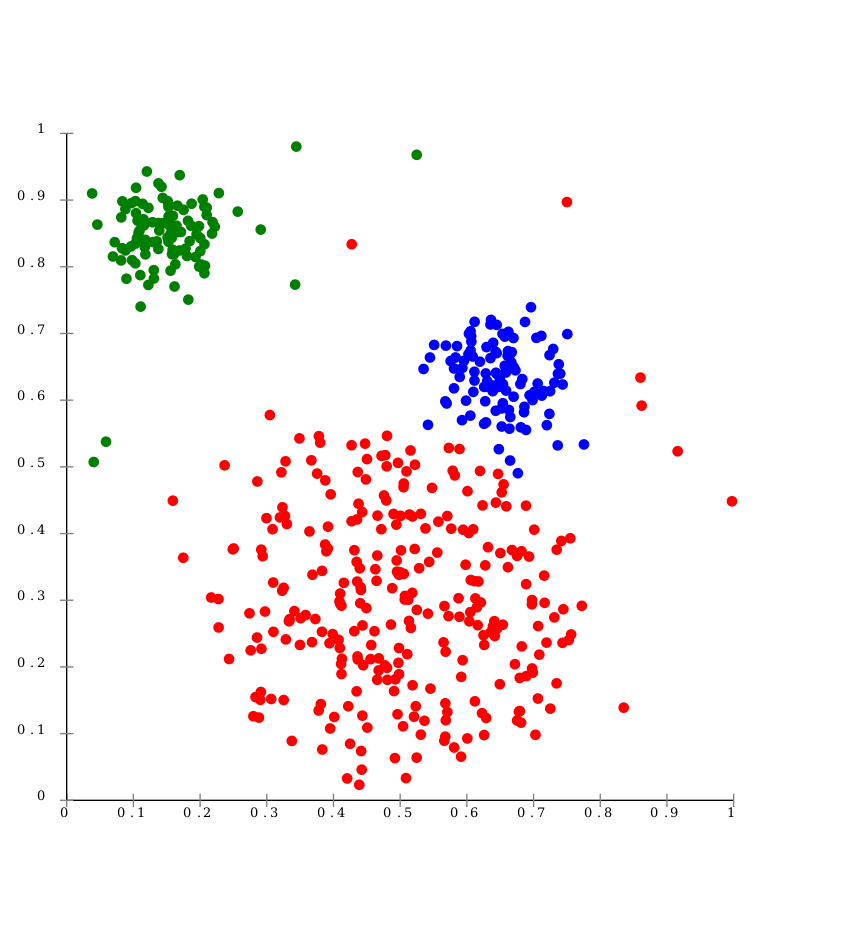
\includegraphics[width=0.4\textwidth, height=0.2\textwidth, center]{images/clust2}
		\item The third is a locality penalty
			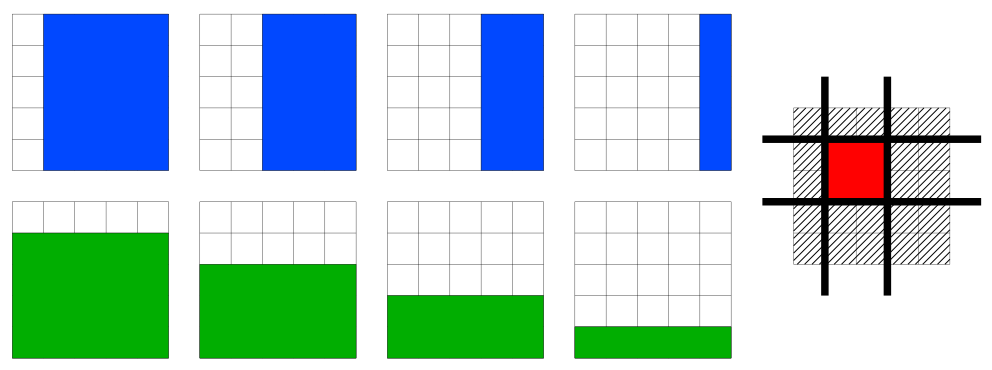
\includegraphics[scale=0.3, center]{images/locality}
	\end{itemize}
\end{frame}

\subsection{Clustering Losses}

\begin{frame}
	\frametitle{Clustering Losses}
	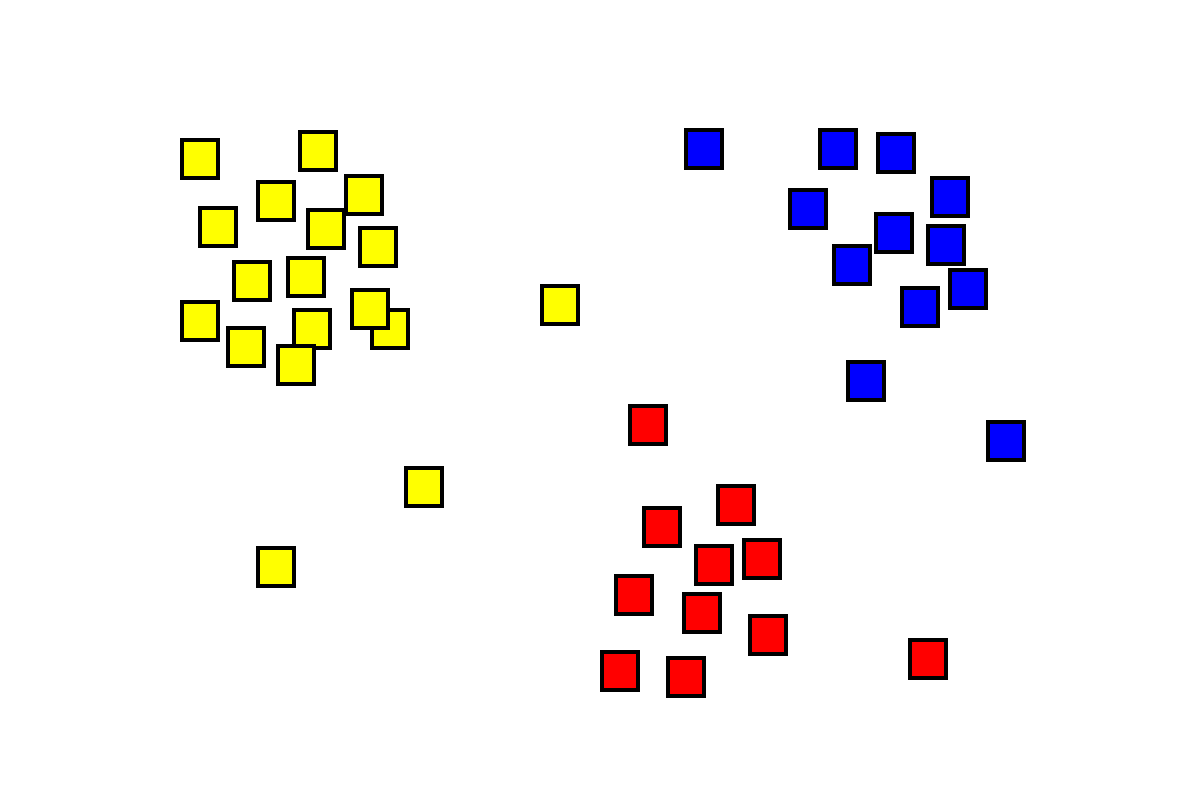
\includegraphics[scale=0.2, center]{images/clust1}
\end{frame}

\begin{frame}
	\frametitle{Mean Entropy Loss}
	\begin{itemize}
		\item The mean entropy loss over a batch of size $T$ is gives by:
			\begin{block}{Mean Entropy Loss (MEL)}
				\begin{equation*}
					J_M = \frac{1}{T}\sum_{t=1}^{T}H(\mathbf{q}_t)
				\end{equation*}
				where $H$ is the entropy and $\mathbf{q}_t = f(\mathbf{X}_t; \Theta)$ is the output
				probability distribution for image $\mathbf{X}_t$
			\end{block}
			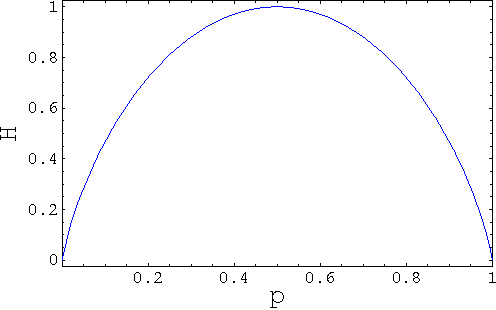
\includegraphics[scale=0.18, center]{images/ent.png}
		\item This increases the confidence of the predicted class
	\end{itemize}
\end{frame}

\begin{frame}
	\frametitle{Negative Batch Entropy Loss}
	\begin{itemize}
		\item The spread of outputs should be similar to the dataset
			label distribution
			\begin{block}{NBEL for Uniform Dataset Label Distribution}
				\begin{equation*}
					J_B = -H(\bar{\mathbf{q}})
				\end{equation*}
				where,
				\begin{equation*}
					\bar{\mathbf{q}} = \frac{1}{T}\sum_{t=1}^{T}\mathbf{q}_t
				\end{equation*}
			\end{block}

	\end{itemize}
\end{frame}

\begin{frame}
	\frametitle{Negative Batch Entropy Loss}
	\begin{itemize}
		\item Can be generalized to any distribution
			\begin{block}{Negative Batch Entropy Loss}
				\begin{equation*}
					\label{eq:nbel}
					J_B = D_{KL} (\bar{\mathbf{q}} \lVert \mathbf{d})
				\end{equation*}
				where $D_{KL}$ is the KL-divergence, and $\mathbf{d}$ is
				the empirical class distribution estimated from $\mathcal{S}$
			\end{block}

	\end{itemize}
\end{frame}


\subsection{Cross Entropy and Clustering}
\begin{frame}
	\frametitle{Adding Cross Entropy Loss}
	\begin{itemize}
		\item For a mini-batch, $\mathcal{B} = \{(\mathbf{X}_k, y_k)\}_{k=1}^R \cup
			\{\mathbf{X}_k\}_{k=R+1}^T$, where $\{(\mathbf{X}_k, y_k)\}_{k=1}^{R} \subseteq
			\mathcal{S}$, and $\{\mathbf{X}_k\}_{k=R+1}^{T} \subseteq \mathcal{U}$, the total loss
			can be give as:
			\begin{block}{Cross Entropy + Clustering}
				\begin{equation*}
					\mathcal{L} = J_C + \alpha J_M + \beta J_B
				\end{equation*}
				\begin{equation*}
					\mathcal{L} = \frac{1}{R} \sum_{t=1}^{R} E_t + \alpha \frac{1}{T}\sum_{t=1}^{T}H(\mathbf{q}_t) +
					\beta D_{KL}(\frac{1}{T}\sum_{t=1}^{T}\mathbf{q}_t \lVert \mathbf{d})
				\end{equation*}
			\end{block}
	\end{itemize}
\end{frame}


%\subsection{Sampling Ratio}
\begin{frame}
	\frametitle{Sampling Ratio}
	\begin{itemize}
		\item Each batch contains both labeled and unlabeled images
		\item Learning depends on their relative importance ($\frac{R}{T}$)
		%\item A higher $\frac{R}{T}$ means that supervised data and losses are considered more
		%	important
	\end{itemize}
\end{frame}


\subsection{Locality Loss}

\begin{frame}
	\frametitle{Locality Loss}
	\begin{itemize}
		\item Consider a class activation map (CAM) \footnote{\tiny{B. Zhou, A. Khosla, A.
				Lapedriza, A. Oliva, and A. Torralba. Learning Deep Features for Discriminative
		Localization.}}, $C \in \mathbb{R}^{N \times N}$. Let $\mathcal{G} = \{g_i
			\subseteq \textrm{support}(C)\}_i$ where $\textrm{support}(C) = [1 \dots N] \times [1
			\dots N]$ and $\cup_{g \in \mathcal{G}} = \textrm{support}(C)$
		\item The following norm induces group sparsity:
	\end{itemize}

	\begin{block}{Sparsity Norm}
		\begin{equation*}
			\Omega (C, \mathcal{G}) = \sum_{g \in \mathcal{G}} \left\lVert C_g \right\rVert _2
		\end{equation*}
		where $C_g$ is the vector formed by the values in $C$ indexed by $g$ and $\left\lVert . \right\rVert_2$ is
		the $L$-$2$ norm.
	\end{block}
\end{frame}


\begin{frame}
	\frametitle{Locality Loss}

	\begin{itemize}
		\item We use four sets $\mathcal G_i = \{g_{ik}\}_{k=1}^N$ corresponding, respectively, to nested
	left-to-right and right-to-left columns, and nested top-to-bottom and bottom-to-top columns,
	\textit{i.e.,}
	\end{itemize}
	\begin{block}{Groups}
		\vspace{-15pt}
		\begin{align*}
			g_{1k} & = [1 \ldots N] \times [1 \ldots k] \\
			g_{2k} & = [1 \ldots N] \times [N-k+1 \ldots N] \\
			g_{3k} & = [1 \ldots k] \times [1 \ldots N] \\
			g_{4k} & = [N-k+1 \ldots N] \times [1 \ldots N]
		\end{align*}
	\end{block}

	\vspace{-10pt}
	\begin{figure}
		\subfigure{
\includegraphics[scale=0.25]{images/g1}}~~
		\subfigure{
\includegraphics[scale=0.25]{images/g2}}~~
		\subfigure{
\includegraphics[scale=0.25]{images/g3}}
	\end{figure}
\end{frame}


\begin{frame}
	\frametitle{Locality Loss}
	\begin{itemize}
		\item The locality-inducing penalty for class $i$ for an image $\mathbf{X}_t$ is:
			\begin{block}{}
				\begin{equation*}
					J_{L,t}^{i} = \sum_{j=1}^{4}\Omega(C^i_t, \mathcal G_j)
				\end{equation*}
				where $C^i_{t}$ is the CAM for class $i$
			\end{block}
		\item Given $\mathbf{q}_t = f(\mathbf{X}_t; \Theta)$, we define our locality-inducing penalty to be
			\begin{block}{}
				\begin{equation*}
					J_{L,t} = \sum_{i} q_{ti} J_{L,t}^i
				\end{equation*}
			\end{block}
		\item The total locality penalty for a batch is $J_L =  \frac{1}{T} \sum_{t=1}^T J_L^t$
	\end{itemize}
\end{frame}

\subsection{Total Loss}
\begin{frame}
	\frametitle{Total Loss}
	\begin{itemize}
		\item Supervised losses (cross-entropy) applied only on labeled data
		\item Unsupervised losses can be applied on both
		\item Our total loss is given as:
	\end{itemize}
	\begin{block}{Total Loss}
		\begin{equation*}
			\mathcal{L} = J_C + \alpha J_M + \beta J_B + \gamma J_L
		\end{equation*}
		where $J_C$ is the cross-entropy loss, $J_M$ is mean entropy loss, $J_B$ is negative batch
		entropy loss, and $J_L$ is the locality loss
	\end{block}
\end{frame}


\section{Experiments}
\begin{frame}
	\frametitle{Experiments}
	\framesubtitle{Test Frame}
	Test
	\begin{itemize}
		\item Test
	\end{itemize}
	\begin{block}{Test}
		Test
	\end{block}
\end{frame}


\section{Conclusion}

Yay!







\end{document}
